\documentclass[conference,a4paper]{IEEEtran}
\usepackage[T1]{fontenc}
\usepackage[utf8]{inputenc}
\usepackage{amsmath,amssymb}
\usepackage{graphicx}
\usepackage{booktabs}
\usepackage{multirow}
\usepackage{array}
\usepackage{url}
\usepackage{cite}
\usepackage{xcolor}
\usepackage[hidelinks]{hyperref}

\newcommand{\code}[1]{\texttt{#1}}
\newcommand{\etal}{\textit{et al.}}

\begin{document}
\hypersetup{
  pdftitle={Evidence-Linked Multi-Recording Conversation Intelligence for Structured Daily Reporting},
  pdfsubject={Mini Project--II research paper},
  pdfkeywords={conversation intelligence, evidence grounding, meeting summarization, provenance}
}


\title{Evidence-Linked Multi-Recording Conversation Intelligence for Structured Daily Reporting}

\author{
\IEEEauthorblockN{[Student Name]}
\IEEEauthorblockA{[Department]\\
Government of Maharashtra's Ismail Yusuf College of Arts, Science and Commerce\\
Jogeshwari (East), Mumbai 400 060, India\\
Affiliated to the University of Mumbai\\
\mbox{[Student Email]}}
\and
\IEEEauthorblockN{[Guide Name]}
\IEEEauthorblockA{[Guide Designation], [Department]\\
Government of Maharashtra's Ismail Yusuf College of Arts, Science and Commerce\\
Jogeshwari (East), Mumbai 400 060, India\\
\mbox{[Guide Email]}}
}

\maketitle

\begin{abstract}
Organizations increasingly record calls and meetings, but the resulting audio rarely
becomes an accountable operational record. Transcription alone preserves words without
extracting tasks, decisions, commitments, dates, or risks, and large language model (LLM)
extraction can produce fluent claims that are not supported by the source. This paper
presents CallMind Intelligence, an end-to-end system that converts multiple independent
recordings into a versioned daily report in which every retained item is linked to a
transcript segment, a verbatim quote, and a timestamp. The system combines validated
multi-file ingestion, provider-routed speech-to-text with segment-level timing, schema-
constrained LLM extraction over eleven insight categories, a strict evidence contract, and
a deterministic cross-recording consolidation stage that preserves source lineage and
surfaces reviewable relationship and conflict proposals. We report a functional and
provenance-oriented evaluation on a frozen deployment: type checking and production build
pass; the offline suite executes 175 tests with 170 passing and five date-sensitive
fixture failures; and a read-only audit of the persisted corpus finds six completed
analyses and five completed reports, with all six per-recording insights and all nine
consolidated evidence items re-validating against stored transcripts, indicating
consistency with the implemented provenance rules rather than semantic accuracy. The study is
deliberately descriptive: the corpus is small, no reference transcripts or human
annotations exist, and no word error rate, precision, recall, or F1 is claimed. The
contribution is a reproducible architecture and an honest account of what such a system
can and cannot yet demonstrate.
\end{abstract}

\begin{IEEEkeywords}
conversation intelligence, evidence grounding, meeting summarization, action-item
extraction, provenance, daily reporting, large language models, speech-to-text.
\end{IEEEkeywords}

\section{Introduction}

Calls, client conversations, and internal meetings are routinely recorded, yet the
operational value of those recordings is usually realized only if someone listens to them
and writes down what matters. Automatic speech recognition (ASR) removes the transcription
bottleneck, but a transcript is not a report: it does not by itself identify who committed
to what, which date changed, which decision was made, or which risk was raised. The
natural next step is to apply large language models (LLMs) to extract structured
information. That step introduces a new risk. An LLM can generate a plausible task or
deadline that no speaker actually stated, and a downstream report can then circulate an
unsupported claim with the same confidence as a supported one.

This paper takes the position that extraction is only useful for operational reporting if
it is \emph{evidence-linked}. Every retained item should point to a specific transcript
segment and a verbatim quote, with timing that can be checked. When several recordings
belong to the same working day, the system should also consolidate them without silently
merging incompatible statements or inventing relationships. These requirements are
system-level: they concern ingestion, queue orchestration, schema design, validation,
consolidation, versioning, and review interfaces, not only a model choice.

We build and study CallMind Intelligence, a MERN/TypeScript prototype that ingests
multiple audio files, transcribes each recording with segment-level timing, extracts typed
insights under a strict JSON schema, validates every insight against its transcript, and
produces a daily report that consolidates insights across recordings. The consolidation
stage is deliberately deterministic rather than LLM-based, so that grouping, relationship
proposals, and conflict detection are inspectable and reproducible. The dashboard is
report-driven and exposes the evidence behind each item.

The paper makes the following contributions:
\begin{enumerate}
\item An evidence contract that persists an insight only when its recording, segment,
quote, and timing resolve against the stored transcript.
\item A deterministic consolidation design that groups by category and normalized subject,
preserves lineage, re-validates evidence, and treats relationships and conflicts as
reviewable proposals rather than automatic truth.
\item A requirements-to-modules mapping across ingestion, transcription, extraction,
consolidation, API, and dashboard layers.
\item A provenance-oriented evaluation protocol and a read-only audit of a frozen
deployment.
\item Explicit limits: corpus size, missing ground truth, sparse extraction, and
date-sensitive test fixtures.
\end{enumerate}

We do not claim that CallMind is the first system of its kind, and we do not report
accuracy metrics that the available data cannot support.

\section{Problem Formulation and Objectives}

\subsection{Inputs and Notation}

Let a workspace contain a set of recordings $R=\{r_1,\dots,r_n\}$. Each recording $r$ has
an immutable audio object and, after transcription, a set of segments
$S_r=\{(s_j,t^{s}_j,t^{e}_j,x_j)\}_{j=1}^{m}$, where $s_j$ is a segment identifier,
$t^{s}_j$ and $t^{e}_j$ are start and end times, and $x_j$ is the segment text. A
recording may also carry speaker labels and a language tag.

An extracted insight is a tuple
\begin{equation}
I=(c,\,x,\,e,\,\kappa,\,\gamma),
\end{equation}
where $c$ is one of eleven categories, $x$ is the content, $\kappa$ is the certainty
(\code{explicit} or \code{inferred}), $\gamma$ is the model confidence, and $e$ is the
evidence tuple
\begin{equation}
e=(r,\,s,\,j,\,t_s,\,t_e,\,q),
\end{equation}
with recording identifier $r$, segment identifier $s$, segment index $j$, start and end
times, and verbatim quote $q$.

\subsection{Evidence Validity}

We say that $e$ is valid for recording $r$ and transcript $S_r$ if and only if
\begin{align}
& r = r^{*},\quad \exists\,(s_j,t^{s}_j,t^{e}_j,x_j)\in S_r \text{ with } s=s_j,\\
& |t_s-t^{s}_j|\le 0.25\,\text{s},\quad |t_e-t^{e}_j|\le 0.25\,\text{s},\\
& \mathrm{norm}(q)\subseteq \mathrm{norm}(x_j),
\end{align}
where $\mathrm{norm}(\cdot)$ lowercases, collapses whitespace, and strips surrounding
punctuation. The identifier and index must agree. An insight whose evidence fails any
condition is rejected rather than stored.

\subsection{Daily Report}

A daily report is
\begin{equation}
D=(\delta,\zeta,\,R_D,\,I_D,\,P_D,\,C_D,\,v,\,\pi),
\end{equation}
where $\delta$ is a calendar date, $\zeta$ is an IANA timezone, $R_D\subseteq R$ is the
source set, $I_D$ is the consolidated insight set, $P_D$ is a set of proposed
relationships, $C_D$ is a set of conflicts, $v$ is a version, and $\pi$ is the previous
version identifier. Every $I\in I_D$ must carry a non-empty lineage
$\Lambda(I)\subseteq R_D$ and at least one valid evidence item. Relationships and
conflicts are proposals: a conflict records incompatible values without deleting either
original claim.

\subsection{Research Objectives}

This work pursues five objectives:
\begin{enumerate}
\item Design and implement an AI-based framework that converts multiple unstructured
audio conversations into structured conversational information.
\item Investigate extraction of tasks, dates, people, decisions, commitments, and other
conversation-derived entities with language models.
\item Implement evidence validation that links each retained insight to a supporting
transcript segment.
\item Develop deterministic consolidation that combines information from multiple
recordings into daily reports while preserving source provenance.
\item Evaluate functional behaviour, evidence traceability, and consolidation capability,
and document the limits of the evaluation.
\end{enumerate}

\subsection{System Requirements and Research Questions}

The system is designed to satisfy seven requirements:
\begin{itemize}
\item[R1] Accept multiple files in one request and report per-file outcomes.
\item[R2] Validate type, size, signature, and content before persistence.
\item[R3] Transcribe with timing suitable for evidence verification.
\item[R4] Extract typed insights under a machine-checkable schema.
\item[R5] Persist an insight only with valid evidence.
\item[R6] Consolidate across recordings deterministically with lineage.
\item[R7] Present a report-driven view with navigable evidence.
\end{itemize}

We pursue three questions. \textbf{RQ1:} How can an end-to-end pipeline enforce
evidence traceability for LLM-extracted operational items? \textbf{RQ2:} How can
multi-recording consolidation remain inspectable and avoid LLM-introduced drift?
\textbf{RQ3:} What can be verified about such a system on a small, frozen deployment
without reference annotations?

\section{Related Work}

\subsection{Review Methodology}

This is a focused narrative literature review, not a systematic literature review. Sources
consulted were ACL Anthology, arXiv, Crossref, and relevant conference proceedings and
publisher records. The search themes were meeting and conversation summarization,
action-item extraction, conversational memory, multi-session conversation understanding,
and source attribution and evidence-grounded information extraction. Papers were selected
for relevance to these themes and to the CallMind problem, not through an exhaustive or
reproducible systematic search. The review therefore does not claim complete coverage of
the field.

\subsection{Meeting Summarization}

Rennard \etal \cite{rennard2023abstractive} survey abstractive meeting summarization and
show that neural encoder--decoder models help but long, multi-party, multi-topic inputs and
evaluation remain difficult. QMSum \cite{zhong2021qmsum} contributes 1,808 query--summary
pairs over 232 meetings, showing that useful summaries are often query-conditioned rather
than generic. Golia and Kalita \cite{golia2023action} drive summarization from detected
action items and report a BERTScore of 64.98 on AMI, about 4.98\% above a fine-tuned BART
baseline. These works establish summarization utility, but their unit is typically one
meeting and their output prose, not an evidence-linked operational record.

\subsection{Action Items and Structured Extraction}

Cohen \etal \cite{cohen2021rephrasing} study rephrasing transcript-derived action items
and show that the task is harder than the analogous email task and benefits from
additional context. Liu \etal \cite{liu2023action} address action-item detection with
regularized context modeling that combines local and global context, and note the scarcity
of annotated action-item data. Together these results motivate a typed extraction schema
and suggest that extraction quality should not be assumed. They do not specify how an
extracted item should be tied back to the exact transcript span that supports it.

\subsection{Multi-Session and Long-Term Conversation}

Conversation Chronicles \cite{jang2023conversation} introduces a one-million-instance
multi-session dataset and a $\sim$630M-parameter model, emphasizing temporal and relational
dynamics across sessions. LoCoMo \cite{maharana2024locomo} evaluates very long-term memory
with dialogues of roughly 600 turns, about 16K tokens, and up to 32 sessions, and finds
that long-context and retrieval augmentation help but do not solve the problem. This line
of work is closest to multi-recording reporting in spirit, but it focuses on dialogue
memory and question answering rather than on producing a dated, reviewable operational
report with per-item provenance.

\subsection{Grounded Attribution and Speech Recognition}

Golany \etal \cite{golany2024mised} generate source-grounded information-seeking dialogs
over meeting transcripts and show that human-verified attribution is valuable and that
fine-tuning on their data improves attribution while reducing annotation effort. Their
result supports the central design choice of this work: grounding is not decorative; it is
a property that must be engineered and checked. Whisper \cite{radford2023whisper}
demonstrates that large-scale weak supervision yields robust ASR across domains, which
makes a provider-routed transcription layer practical.

\subsection{Positioning}

Table~\ref{tab:related} summarizes the comparison. The reviewed work provides strong
methods for summarization, action-item detection, multi-session memory, and attribution,
but these strands are usually separate and assume a single meeting, synthetic dialogue, or
modelling benchmark. Within the selected literature, we did not find an end-to-end system
combining per-recording evidence-linked extraction with cautious cross-recording
daily-report consolidation and provenance-preserving review. This is a scoped finding, not
a claim that no such system exists.

\begin{table*}[t]
\centering
\caption{Positioning against the reviewed literature.}
\label{tab:related}
\setlength{\tabcolsep}{5pt}
\footnotesize
\renewcommand{\arraystretch}{1.15}
\begin{tabular}{@{}>{\raggedright\arraybackslash}p{0.9cm}>{\raggedright\arraybackslash}p{3.3cm}>{\raggedright\arraybackslash}p{3.3cm}>{\raggedright\arraybackslash}p{3.1cm}>{\raggedright\arraybackslash}p{2.4cm}>{\raggedright\arraybackslash}p{2.2cm}@{}}
\toprule
Ref. & Focus & Data / scale & Evidence or attribution & Multi-recording & Structured output \\
\midrule
\cite{rennard2023abstractive} & Abstractive meeting summarization (survey) & Multiple meeting corpora & Discussed as evaluation issue & No & Prose summary \\
\cite{zhong2021qmsum} & Query-based meeting summarization & 1,808 pairs / 232 meetings & Query-conditioned summaries & No & Prose summary \\
\cite{golia2023action} & Action-item-driven summarization & AMI & BERTScore 64.98 & No & Summary \\
\cite{cohen2021rephrasing} & Rephrasing transcript action items & Transcript/email pairs & Context-conditioned generation & No & Rephrased item \\
\cite{liu2023action} & Action-item detection & Meeting transcripts & Local + global context & No & Item labels \\
\cite{jang2023conversation} & Multi-session dialogue & 1M instances & Temporal/relational context & Sessions, not reports & Dialogue \\
\cite{maharana2024locomo} & Very long-term memory & $\sim$600 turns, up to 32 sessions & Long-context / RAG analysis & Sessions, not reports & QA \\
\cite{golany2024mised} & Source-grounded dialogs & Meeting transcripts & Human-verified attribution & No & Dialog with sources \\
\textbf{Ours} & Evidence-linked reporting & 8 recordings (audit) & Segment, quote, timing & Yes & Typed insights/report \\
\bottomrule
\end{tabular}
\end{table*}

\section{System Design and Methodology}

\subsection{Architecture and Data Flow}

Figure~\ref{fig:arch} shows the pipeline. A multi-file upload enters validation and
deduplication; accepted recordings receive immutable storage keys and are enqueued for
preparation. Transcription is routed by language hint, and the timed transcript feeds
schema-constrained extraction. Validated insights are stored per recording. A daily-report
request selects eligible recordings, consolidates insights deterministically, re-validates
evidence, and persists a versioned report. The web client reads reports and opens an
evidence drawer that navigates to the exact recording and segment.

\begin{figure*}[t]
\centering
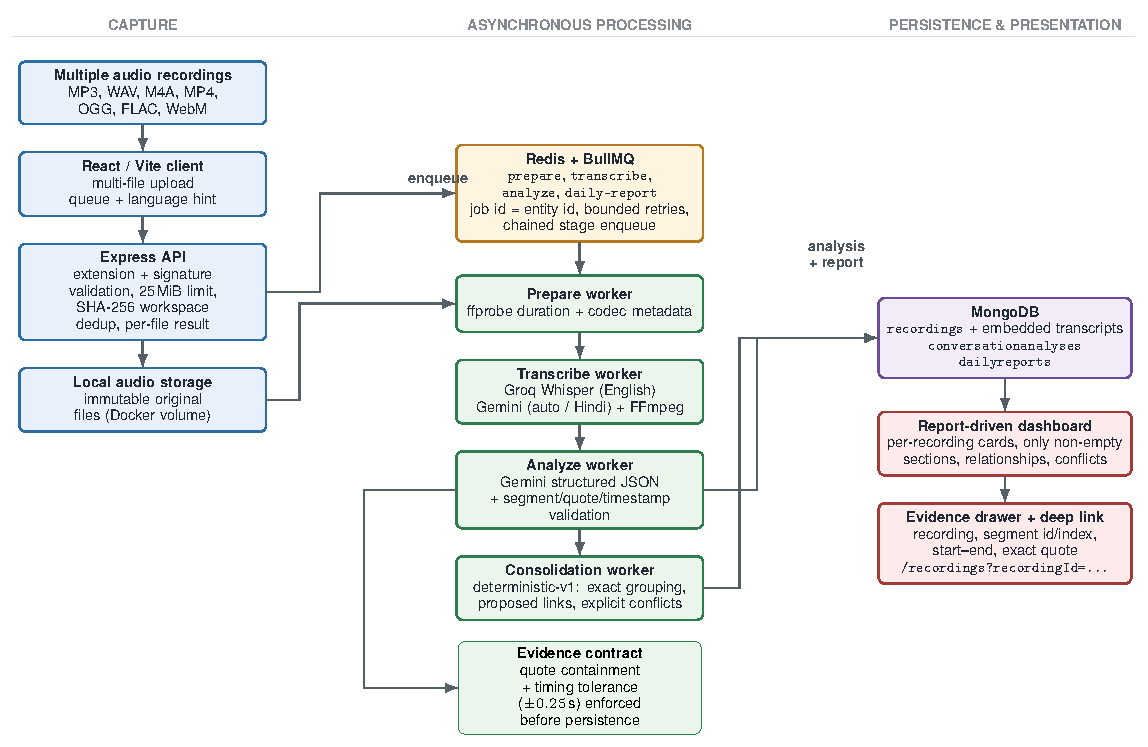
\includegraphics[width=0.94\textwidth]{figures/architecture.pdf}
\caption{System architecture. Arrows show the recording pipeline from ingestion through
transcription, extraction, and deterministic consolidation to persistence and report
presentation. Every persisted insight carries an evidence tuple that is validated
against the stored transcript before it can reach a report.}
\label{fig:arch}
\end{figure*}

\subsection{Ingestion and Validation}

The upload endpoint accepts up to 20 files per request and returns a per-file result:
\code{created}, \code{duplicate}, or \code{rejected}. A batch is therefore not lost because
one file is malformed. Validation checks the extension allow-list, non-empty size, a
25\,MiB per-file limit, the detected container signature, and agreement between the
detected MIME type and the extension. ASF/WMA containers are rejected. A SHA-256 checksum
scoped to the workspace provides idempotency, backed by a unique index; a duplicate returns
the existing recording rather than creating a second copy. Accepted files are moved from a
temporary directory into workspace-scoped immutable storage. The recording then advances
through explicit states: \code{uploaded}, \code{ready\_for\_transcription},
\code{transcribing}, \code{transcribed}, \code{analyzing}, \code{analysis\_completed}, or a
failure state with a typed error code.

\subsection{Provider-Routed Transcription}

Language routing is explicit. An English hint (\code{en}) selects Groq's
\code{whisper-large-v3-turbo}; \code{auto} and Hindi (\code{hi}) select Gemini's
\code{gemini-3.5-transcribe} with diarization and word-level timestamps. When a container
is not accepted by the selected provider, the worker transcodes a temporary 16\,kHz mono
WAV with FFmpeg and removes the temporary directory afterwards. The transcript stores
segments, optional speaker labels, and timing. The timing is not cosmetic: it is the
substrate for the evidence check in the next stage.

\subsection{Evidence-Linked Extraction}

Extraction uses Gemini structured output with a JSON response schema, temperature 0.2, and
a 120\,s timeout. A primary model and a fallback model are configured; each model receives
bounded retries with exponential backoff, and provider errors are mapped and redacted
before logging. The schema defines eleven categories: topic, person, task, date, decision,
commitment, transaction, project, risk, question, and a generic insight. Each item carries
content fields, a certainty label (\code{explicit} or \code{inferred}), an optional
confidence, and an evidence object.

The evidence check is the core of the design. The validator resolves the recording and
segment, checks identifier/index agreement, verifies that the quote is contained in the
segment text after normalization, and verifies that the reported start and end times are
within 0.25\,s of the segment. Items that fail are rejected; content-free items are
dropped. This makes fabrication detectable at write time rather than after a report has
been circulated. It is a necessary but not sufficient condition: quote containment does
not prove that the quote entails the claim, a limitation we return to in
Section~\ref{sec:threats}. Figure~\ref{fig:prov} summarizes the resulting chain from
transcript segment to persisted analysis and consolidated report.

\begin{figure*}[t]
\centering
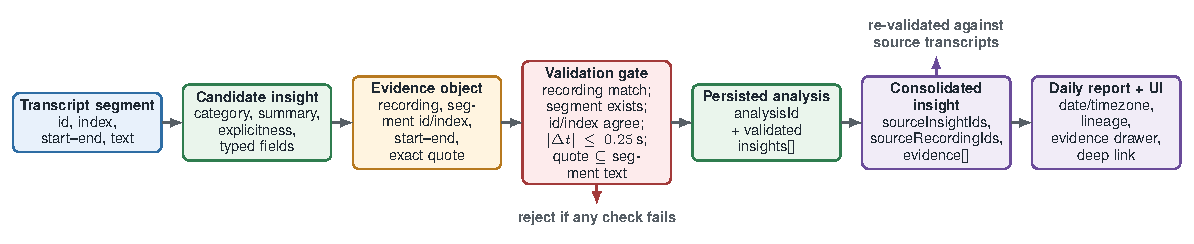
\includegraphics[width=0.90\textwidth]{figures/provenance.pdf}
\caption{Evidence-provenance chain. A candidate insight is persisted only if the validation
gate resolves its recording and segment, checks identifier/index agreement, quote
containment, and timing within $\pm0.25$\,s. Consolidated insights retain source lineage
and are re-validated against the source transcripts.}
\label{fig:prov}
\end{figure*}

\subsection{Deterministic Consolidation}

Daily-report consolidation is deterministic (\code{deterministic-v1}) and does not call an
LLM. Insights from the selected recordings are grouped by category and a normalized
subject/entity key. Within a group, the consolidation preserves the union of source insight
identifiers and source recording identifiers and retains the evidence items. The
consolidated evidence is re-validated against the source transcript before the report is
marked complete. Relationships are proposed only under explicit rules: shared entity,
shared topic, task update, deadline revision, and value revision. Each relationship starts
as \code{pending}. Selected rule-based conflict detection is implemented for status, date,
and quantity disagreements; each conflict starts as \code{unresolved} and can later be
resolved or dismissed without deleting the original values. The design trades recall for
inspectability: it does not perform fuzzy entity resolution, so similar names are
deliberately not merged. The system does not claim to detect all forms of contradiction.

\subsection{Report API, Versioning, and Dashboard}

A report request supplies explicit recording identifiers, a \code{YYYY-MM-DD} date, and an
IANA timezone. Eligibility requires \code{analysis\_completed} status, a linked transcript,
and a recording creation instant inside the selected local date. In the present
implementation, report-date eligibility is determined using the recording creation
timestamp and the specified IANA timezone. The actual conversation date is not
independently inferred or validated. A request fingerprint rejects an identical duplicate
request. Regeneration creates a new version linked to the
previous report, so the history is append-only. The dashboard is read-only and
report-driven: it renders one card per source recording, shows only non-empty category
sections, polls while a report is active, and lets a reviewer open an evidence drawer. A
deep link carries the recording, segment identifier, segment index, and start time to the
recordings view. The interface therefore treats a report as a set of claims with sources,
not as a generated paragraph.

\begin{table*}[t]
\centering
\caption{Implementation mapping from requirements to mechanisms and primary modules.}
\label{tab:impl}
\footnotesize
\renewcommand{\arraystretch}{1.15}
\begin{tabular}{@{}>{\raggedright\arraybackslash}p{0.7cm}>{\raggedright\arraybackslash}p{5.4cm}>{\raggedright\arraybackslash}p{8.6cm}@{}}
\toprule
Req. & Mechanism & Primary modules \\
\midrule
R1 & Per-file outcome in a multi-file upload & \code{apps/api/src/routes/recordings.ts}; shared upload schemas \\
R2 & Extension, size, signature, MIME, and ASF/WMA checks & \code{audioValidation.ts}; recording constants \\
R3 & Language routing; diarization; word timestamps; FFmpeg transcode & \code{stt.ts}; \code{groqTranscription.ts}; \code{geminiTranscription.ts} \\
R4 & JSON response schema; 11 categories; primary/fallback; retries & \code{analysis.ts}; \code{geminiAnalysis.ts}; worker env config \\
R5 & Segment resolution; quote containment; $\pm0.25$\,s timing; rejection & \code{conversationAnalysis.ts}; \code{recordingAnalyze.ts} \\
R6 & Category/key grouping; lineage; relationships; conflicts; re-validation & \code{reportConsolidation.ts}; \code{dailyReports.ts} constants \\
R7 & Report-driven cards; evidence drawer; deep links; polling & \code{dashboard.tsx}; \code{evidence-drawer.tsx}; \code{recording-deep-link.ts} \\
\bottomrule
\end{tabular}
\end{table*}

\section{Implementation}

The system is a TypeScript monorepo with five workspaces: \code{shared} (schemas,
constants, validation), \code{db} (Mongoose models and indexes), \code{api} (Express),
\code{worker} (BullMQ processors), and \code{web} (React 18, Vite, Tailwind, and
shadcn-compatible components). MongoDB stores recordings, transcripts, analyses, and
reports. Redis and BullMQ provide four queues: prepare, transcribe, analyze, and
daily-report. Jobs use entity identifiers as job identifiers, claim work atomically to
avoid double processing, and use bounded exponential retries (three attempts for prepare,
transcribe, and daily-report; two for analyze; 5\,s base delay). Worker concurrency is two
for prepare, transcribe, and analyze, and one for daily-report. Docker Compose runs the
five services. Authentication and cloud object storage are intentionally out of scope, and
the worker calls provider APIs directly rather than through a routing intermediary.

Table~\ref{tab:impl} maps the seven requirements to mechanisms and modules. The mapping is
included because the contribution is architectural: the evidence contract is enforced by
cooperating components, not by a single prompt.

\section{Experimental Setup and Evaluation Methodology}

\subsection{Frozen Boundary and Environment}

The implementation was frozen at the end of the daily-report phase, before the next planned
phase. No prompt, schema, provider, model, application file, test, persisted record, or
container was modified during evaluation. No live Groq or Gemini inference was performed during
evaluation, no production queue job was triggered, and no database write was issued. The environment
was Node 24.15.0, npm 11.12.1, Docker 29.5.2, and Docker Compose 5.1.4 on Linux. The API
health endpoint reported the API, MongoDB, and Redis as up.

\subsection{Evaluation Corpus}

The evaluation uses a small functional smoke-test corpus from one deployment: eight
recordings, six completed analyses, seven transcripts, and five completed daily reports.
Audio durations are approximately 1.7--44\,s. Six transcripts came from Groq's
\code{whisper-large-v3-turbo} and one from Gemini's \code{gemini-3.5-transcribe}; language
tags were \code{English} (five), ``Hindi'' (one), and \code{hi} (one). No ground-truth
labels or reference transcripts exist. The corpus exercises the pipeline and provenance
contract; it is not a representative benchmark and does not establish general-purpose
accuracy or effectiveness.

\subsection{Verification Procedure}

We ran the repository's type checker and production build, then the offline test suites per
workspace so that counts could be attributed. The daily-report suites use an in-memory
MongoDB and mocked providers; they do not require live credentials. We then performed a
read-only audit of the persisted corpus with \code{mongosh} queries and a script that
re-applied the evidence rules to stored insights and consolidated evidence. No identifiers,
filenames, phone numbers, names, or transcript text were extracted for publication.

\subsection{Metrics}

Three kinds of measurement are reported. \emph{Functional verification} is binary:
typecheck, build, and test outcomes. \emph{Provenance validity} is the fraction of stored
items whose evidence satisfies the contract in Section~II-B; this is an internal
consistency measure, not a semantic-correctness measure. \emph{Descriptive coverage}
counts recordings, analyses, insights, categories, reports, relationships, and conflicts.
We do not compute word error rate, character error rate, precision, recall, F1, or
calibration, because the corpus has no reference transcripts or human relevance
judgements. Model confidence values are reported only as observed metadata.

\subsection{Baselines}

Because no annotated benchmark exists, we compare capabilities qualitatively rather than
by score. The first baseline is a transcript-only workflow: a reviewer reads or searches
the transcript. The second is independent per-recording summarization: each recording
produces a prose summary with no shared schema and no cross-recording consolidation. The
proposed system is compared on traceability, structured output, cross-recording
consolidation, conflict handling, and review effort. This comparison is a design argument,
not an empirical result, and is labelled as such.

\section{Results and Discussion}

\subsection{Static and Test Results}

Type checking passed, and the production build completed with a 397.84\,kB JavaScript
bundle (121.04\,kB gzip). The offline suite executed 30 files and 175 tests: 170 passed and
five failed (Table~\ref{tab:tests}). All five failures are in the daily-report suites and
share one cause. The fixtures create recordings without an explicit creation time, so the
records default to the audit date, while the fixture report date is hard-coded to an
earlier day. Source validation correctly rejects them as outside the reporting date. This
is a fixture defect, not a live-product regression observed in this audit, and the fixtures
were not modified. The \code{api} and \code{worker} test commands therefore exit non-zero.

\begin{table}[t]
\centering
\caption{Offline test results by workspace (25 November 2026).}
\label{tab:tests}
\small
\renewcommand{\arraystretch}{1.1}
\begin{tabular}{@{}lrrrr@{}}
\toprule
Workspace & Files & Tests & Pass & Fail \\
\midrule
\code{shared} & 5 & 21 & 21 & 0 \\
\code{db} & 1 & 5 & 5 & 0 \\
\code{api} & 4 & 32 & 29 & 3 \\
\code{worker} & 11 & 46 & 44 & 2 \\
\code{web} & 9 & 71 & 71 & 0 \\
\midrule
Total & 30 & 175 & 170 & 5 \\
\bottomrule
\end{tabular}
\end{table}

\subsection{Persisted Corpus}

Table~\ref{tab:corpus} summarizes the read-only audit. It found eight recordings, of which
six had completed analyses, one was transcribed but not analyzed, and one was prepared but
not transcribed. Five daily reports were completed. All six analyses used
\code{gemini-3.1-flash-lite} with the fallback flag set and \code{gemini-3.8-flash}
attempted first; the persisted result therefore came from the fallback model in every
case. This is a factual observation about the stored records, not a controlled comparison
of the two models.

Extraction was sparse: the six analyses contained six insights in total, distributed as
0, 0, 1, 1, 2, and 2 per analysis. Five were categorized as the generic \code{insight} and
one as \code{date}; all six were marked \code{explicit}; one had high confidence and five
had no confidence value. On this sample the extractor demonstrates the contract rather than
extraction quality.

\begin{table}[t]
\centering
\caption{Evidence-traceability audit on the persisted corpus.}
\label{tab:evidence}
\small
\renewcommand{\arraystretch}{1.1}
\begin{tabular}{@{}lrr@{}}
\toprule
Check & Passed & Total \\
\midrule
Per-recording insights checked & -- & 6 \\
Segment resolved & 6 & 6 \\
Quote contained in segment & 6 & 6 \\
Timing within $\pm0.25$\,s & 6 & 6 \\
All checks passed & 6 & 6 \\
\midrule
Consolidated evidence re-validated & 9 & 9 \\
\bottomrule
\end{tabular}
\end{table}

\subsection{Evidence Traceability}

Table~\ref{tab:evidence} reports the central result. Every one of the six stored insights
resolved to a real segment, had a quote contained in that segment after normalization, and
had timing within 0.25\,s. Every one of the nine consolidated evidence items also
re-validated against its source transcript. On this corpus, the evidence contract held
without exception. This is the property the architecture was designed to enforce, and it is
the strongest empirical statement the current data supports. The 6/6 and 9/9 results
indicate consistency with the implemented provenance rules. They should not be interpreted
as 100\% extraction accuracy or proof that the corresponding insights are semantically
correct. The audit re-applied the implementation's validation rules; it was not an
independent human evaluation. Quote containment and timing establish internal traceability,
not semantic entailment: a supporting quote can exist while the extracted interpretation is
still incorrect or incomplete.

\subsection{Daily Reports and Consolidation}

The five reports comprised two in UTC and three in \code{Asia/Kolkata}. Across them there
were seven source-recording links, nine consolidated insights, and one regenerated version
with a previous-report link. Two reports consolidated two recordings and three insights
each; the others had one source with two, one, and zero insights. The consolidated insights
were all in the generic category. No relationships and no conflicts were produced. In the
present implementation, selected rule-based conflict detection covers status, date, and
quantity disagreements, and relationship proposals are generated only by explicit rules.
The absence of relationships and conflicts is consistent with both the small, weakly
overlapping sample and the conservative exact-match design. It means the relationship and
conflict paths are verified by unit tests and code inspection, not by this dataset. We make
no general claim about relationship or conflict detection accuracy, and the system does not
claim to detect all forms of contradiction.

\begin{table}[t]
\centering
\caption{Persisted-corpus summary (read-only audit).}
\label{tab:corpus}
\small
\renewcommand{\arraystretch}{1.1}
\begin{tabular}{@{}lrr@{}}
\toprule
Quantity & Observed & Notes \\
\midrule
Recordings & 8 & 6 analyzed \\
Transcripts & 7 & 6 Groq, 1 Gemini \\
Completed analyses & 6 & all fallback model \\
Extracted insights & 6 & 0--2 per analysis \\
Completed reports & 5 & 2 UTC, 3 IST \\
Source links & 7 & across reports \\
Consolidated insights & 9 & all generic \\
Validated consolidated evidence & 9/9 & re-checked \\
Relationships & 0 & none proposed \\
Conflicts & 0 & none detected \\
\bottomrule
\end{tabular}
\end{table}

\subsection{Capability Comparison}

Table~\ref{tab:baseline} contrasts the workflows. A transcript-only workflow preserves
everything but requires a human to find and reconcile items. Independent per-recording
summaries improve readability but produce no shared schema, no cross-recording lineage, and
no systematic conflict handling. The proposed system adds typed items, per-item evidence,
deterministic consolidation, and a review interface, at the cost of recall on this small
sample and of engineering complexity. The comparison is qualitative; it does not quantify
review time or summary quality.

\begin{table}[!t]
\centering
\caption{Qualitative capability comparison. This is a design comparison, not a measured
benchmark.}
\label{tab:baseline}
\footnotesize
\setlength{\tabcolsep}{3pt}
\renewcommand{\arraystretch}{1.12}
\begin{tabular}{@{}>{\raggedright\arraybackslash}p{2.5cm}>{\raggedright\arraybackslash}p{1.65cm}>{\raggedright\arraybackslash}p{1.65cm}>{\raggedright\arraybackslash}p{2.1cm}@{}}
\toprule
Capability & Transcript only & Per-recording & Proposed \\
\midrule
Typed output & No & No & Yes, 11 types \\
Per-item evidence & Raw text search & Usually none & Segment, quote, time \\
Cross-recording merge & Manual & Manual & Deterministic groups \\
Source lineage & Manual & Weak & IDs + evidence \\
Conflict handling & Manual & Usually absent & Reviewable \\
Report versioning & Ad hoc & Ad hoc & Append-only \\
Review interface & Text search & Summary list & Cards + evidence \\
Measured accuracy & Not measured & Not measured & Not measured \\
\bottomrule
\end{tabular}
\end{table}

\subsection{Discussion}

Three findings stand out. First, the evidence contract is enforceable in practice: all
stored items re-validated, including consolidated items, which shows that re-checking at
consolidation time is feasible and catches lineage mistakes. This is a statement about
provenance consistency, not semantic correctness. Second, schema-constrained
extraction can still be sparse and generic. The model returned few items and mostly used
the fallback category, so a system that advertises typed extraction must report category
coverage rather than assume it. Third, deterministic consolidation makes the report
auditable but limits recall: exact normalized keys will miss paraphrases and aliases, and a
conservative relationship policy will produce few proposals. These are design trade-offs
that a larger, annotated study should quantify.

The date-sensitive test failures are also informative. They show that date and timezone
scoping is not a cosmetic filter; it is a correctness boundary. Report-date eligibility is
based on the recording creation timestamp and the requested IANA timezone; the actual
conversation date is not independently inferred or validated. This is a report-scoping
date, not necessarily the conversation date, so uploading on a different day can mis-scope
a recording. A production system should carry an explicit conversation timestamp.

\section{Threats to Validity and Limitations}
\label{sec:threats}

\emph{Construct validity.} Evidence validity checks quote containment and timing, not
semantic entailment. A quote can be present yet fail to support the claim, or support it
only under context the report omits. The contract is necessary but not sufficient.
Consolidation groups by exact normalized keys, so it under-merges paraphrases and aliases.
Report-date eligibility uses recording creation time rather than an inferred conversation
date, so upload timing can mis-scope a recording.
\emph{Internal validity.} The five test failures are fixture defects, but they mean the
root suite is not green; a reader should not treat the test count as a quality score. The
persisted analyses all used the fallback model, so primary-model behaviour is not
characterized. \emph{External validity.} The corpus is eight short recordings (roughly 1.7
to 44 seconds) from a single deployment; it is not representative of long meetings,
multi-party calls, code-switching, or noisy telephony. \emph{Statistical conclusion
validity.} With no reference transcripts or annotations, no accuracy metric is estimable.
The observed 6/6 and 9/9 provenance rates are descriptive and have wide uncertainty.
\emph{Scope.} Authentication, tenant isolation, cloud storage, and provider-cost control
are not evaluated. ASR errors propagate into extraction, and the system does not correct
them. Finally, no live provider call was made during evaluation, so provider drift and
latency under load are not measured.

\section{Conclusion and Future Scope}

We presented CallMind Intelligence, an evidence-linked pipeline that turns multiple
recordings into a versioned daily report. The design enforces a per-item evidence contract,
uses schema-constrained extraction over eleven categories, consolidates deterministically
with lineage, and exposes evidence through a report-driven interface. On a frozen
deployment, type checking and the production build passed, 170 of 175 offline tests passed,
and a read-only audit found that all six stored insights and all nine consolidated evidence
items re-validated against their transcripts, which indicates consistency with the
provenance rules rather than extraction accuracy. The same audit exposed the limits: a small
short-recording corpus, sparse and mostly generic extraction, a fallback-only analysis
snapshot, no observed relationships or conflicts, and five date-sensitive test failures.
We therefore report a reproducible architecture and a provenance result, not an accuracy
claim.

Future work has four directions. First, annotate a held-out set of recordings to estimate
word error rate, evidence-level precision and recall, and category-wise extraction quality,
and to compare against transcript-only and per-recording-summary baselines. Second, add
semantic entailment checking and fuzzy entity resolution while preserving the deterministic
audit trail. Third, carry an explicit conversation timestamp and support speaker-aware
consolidation. Fourth, add authentication, tenant isolation, and a human review workflow
for relationships and conflicts. A larger study should also measure review time and
provider cost, which the present audit does not cover.

\section*{Acknowledgment}

The authors thank the department and the project reviewers for their support and
feedback.

\bibliographystyle{IEEEtran}
\bibliography{references}

\end{document}
